% !TEX root = ../preview.tex

\section{Auxiliary Video-Codec Diagnostic}
\label{app:wan-video-codec-diagnostic}

To isolate how temporal feedback coverage interacts with the video codec, we
additionally apply state-only FBFM to the auxiliary ball-meets-ball sequence.
This diagnostic is separate from the primary robot evaluation and exposes an
unresolved behavior that appears when feedback measurements cover only a
finite prefix of a temporally compressed video latent.

Extending feedback from 10 to 30 time-aligned slots progressively covers the
measured motion. With all 30 slots, FBFM reduces table-region MAE from 21.77 to
6.34 and reduces the mean orange-ball center error from 173.84 to 3.05 pixels,
confirming that the state constraints affect the generated trajectory. The
principal failure mode is instead the large-area corruption that develops after
the finite feedback horizon in the 10- and 20-slot settings. Its onset moves
later as the measured prefix is extended, while full 30-slot coverage largely
preserves the scene structure over the evaluated horizon.

\begin{figure*}[t]
    \centering
    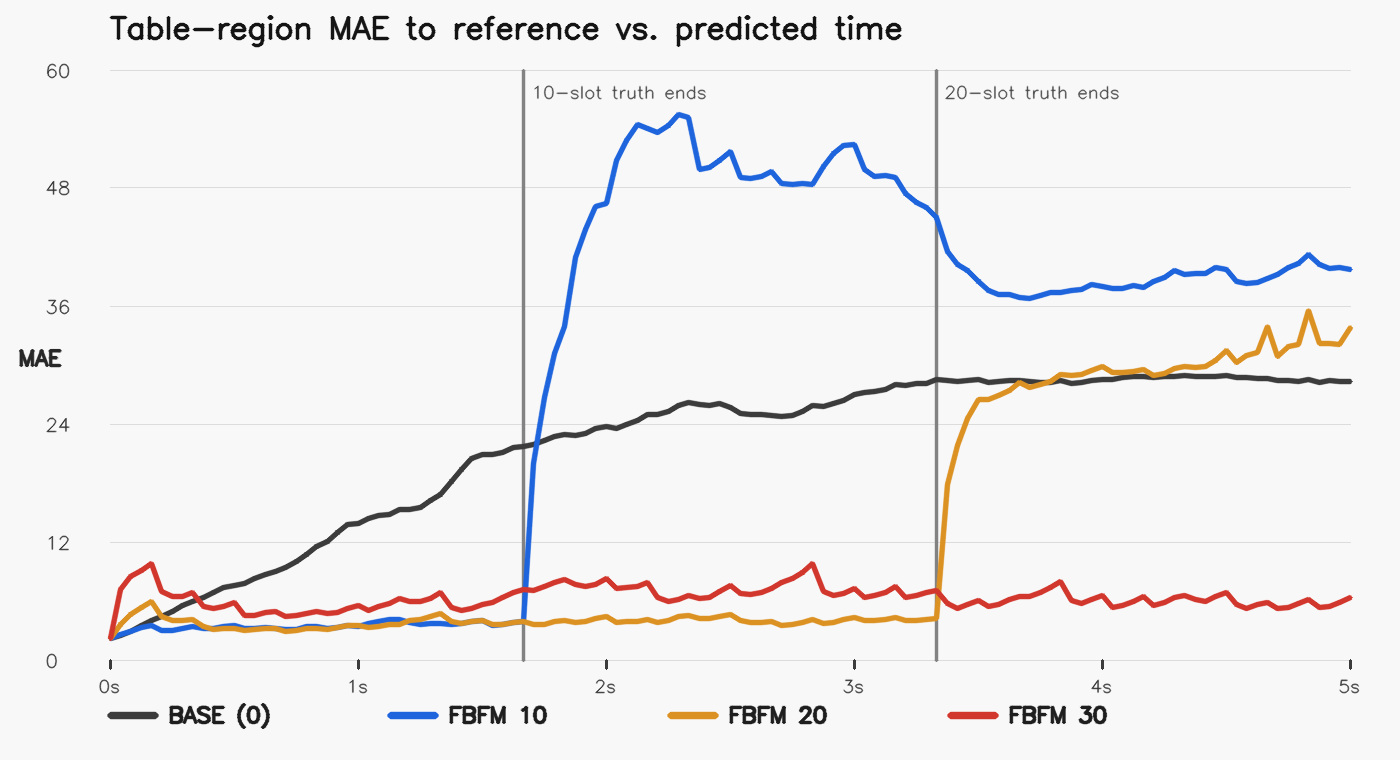
\includegraphics[width=0.9\textwidth]{../material/wan2.2/slot_ablation_mae_curve.png}
    \caption{Image-space error under finite feedback coverage. Curves report
    the frame-wise table-region MAE, and vertical lines mark the ends of the
    measured prefixes for the 10- and 20-slot settings.}
    \label{fig:wan-slot-ablation-mae}
\end{figure*}

The error rise aligns closely with the end of each measured prefix: the 10-slot
curve increases after approximately 1.67~s, the 20-slot curve after
approximately 3.33~s, and the 30-slot curve remains low when feedback spans the
full evaluated horizon. This curve documents a temporal association between
feedback coverage and the failure onset, but does not identify its mechanism.

One possible explanation is a Wan2.2-specific mismatch between the codec and
the generative backbone. Pseudoinverse guidance assumes that a measurement
lifted through the encoder is compatible with the model's clean latent-state
distribution. Wan2.2's joint video training and subsequent post-training may
alter the effective VAE-latent distribution used by the generator, such that
independently encoded observations do not necessarily remain semantically
meaningful clean-video states under the guided dynamics. Once the finite
constraint ends, such a mismatch could amplify and decode into large regions
without a coherent visual interpretation. We leave this as a model-specific
hypothesis: establishing the causal mechanism would require controlled
image-/latent-space diagnostics and codec retraining experiments beyond the
scope of this paper.

\begin{figure*}[p]
    \centering
    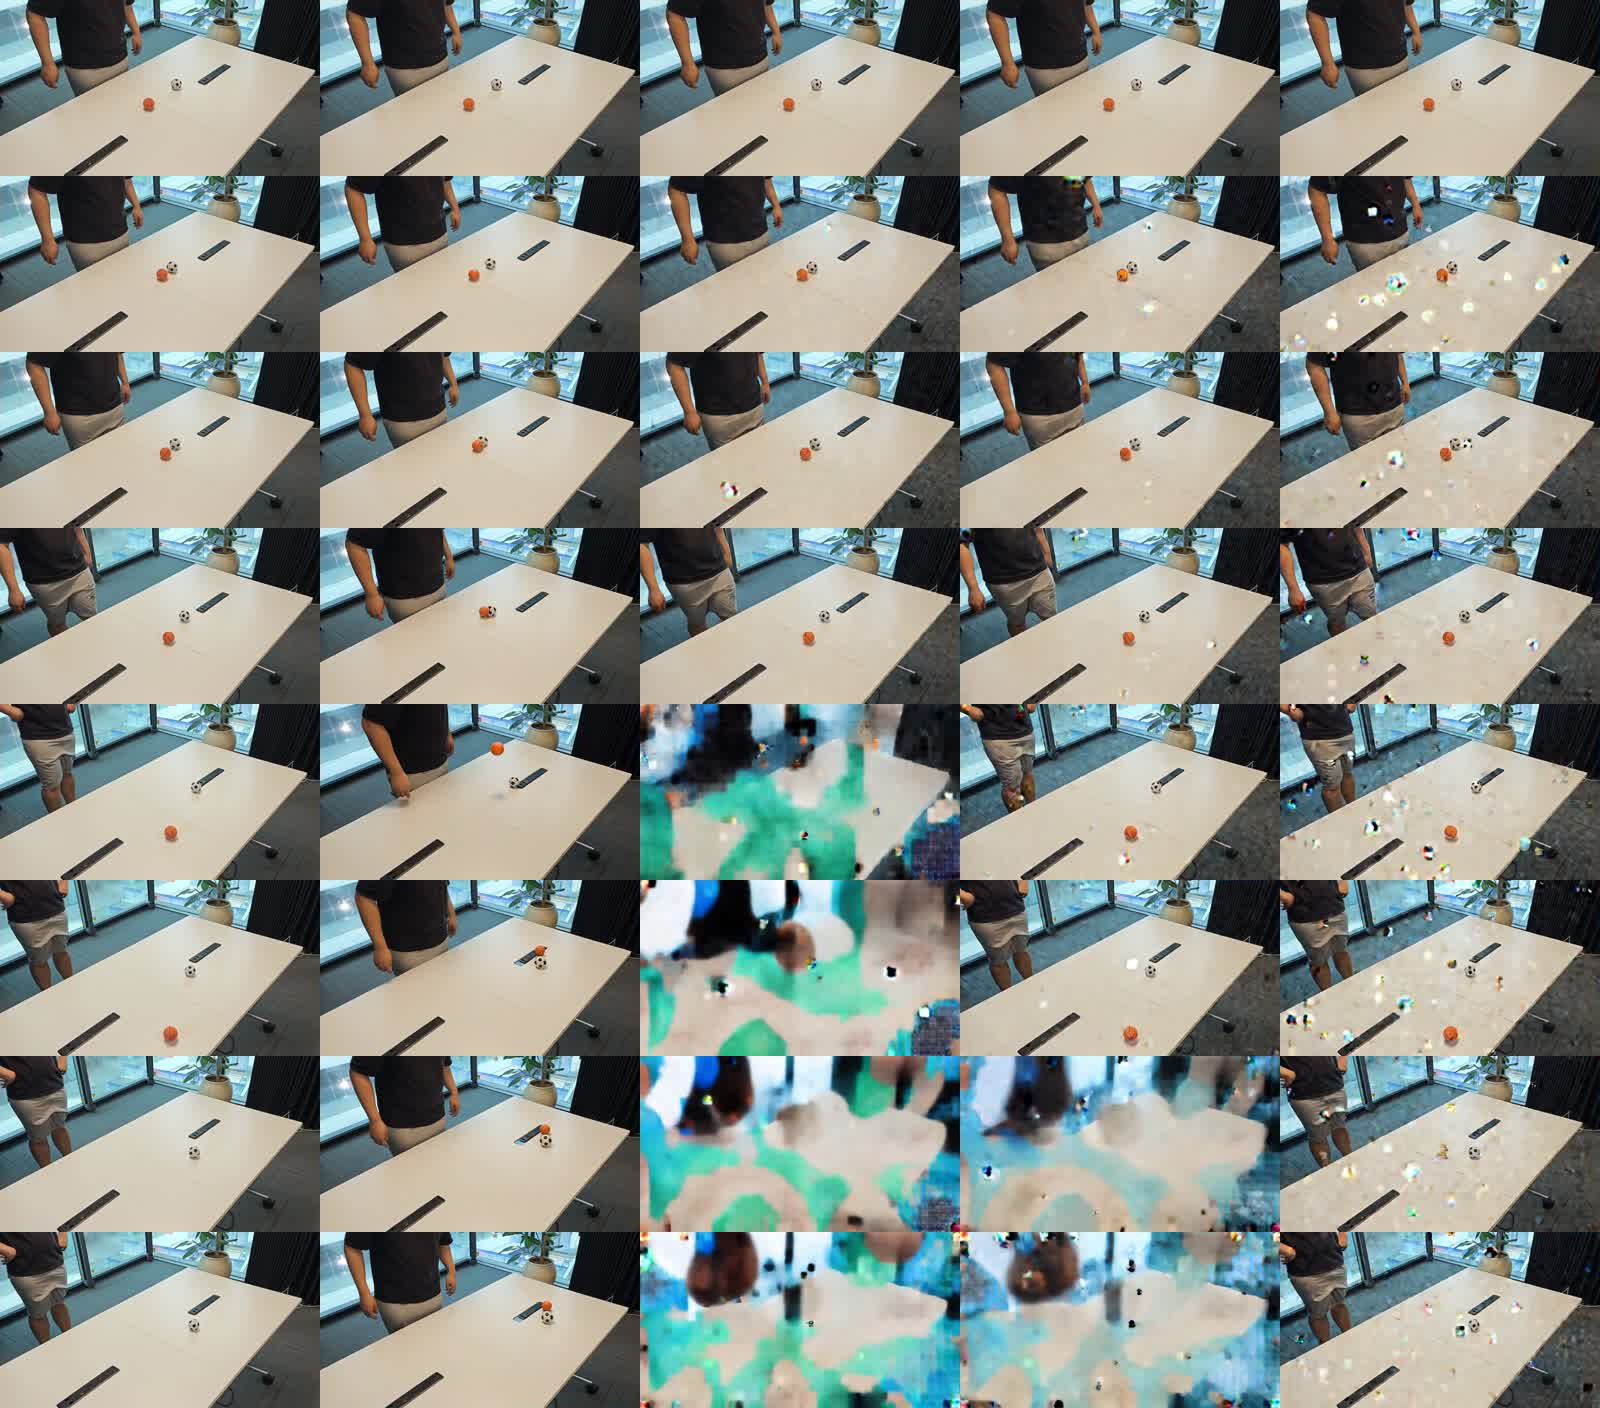
\includegraphics[width=\textwidth]{../material/wan2.2/ball_meet_ball_fiveway_vertical.jpg}
    \caption{State-feedback coverage on the auxiliary ball-collision sequence.
    Rows show 0, 0.25, 0.5, 1, 2, 3, 4, and 5~s; columns show the reference,
    Wan2.2 Base, and FBFM with 10, 20, and 30 measured latent slots.}
    \label{fig:wan-ball-meet-ball}
\end{figure*}
